\documentclass{article}
\usepackage[margin=1in]{geometry}
\usepackage{graphicx}
\usepackage{titling}

\setlength{\droptitle}{-10em}  

\title{Caf\'{e} Eatcon - An Educational Economics Game}
\author{Adam Bilbeano, David Chapman, Hannah Pruse, Sol Joye}
\date{}

\begin{document}
\maketitle

\section{Team Members and Roles}
\begin{center}
\begin{tabular}{|c|c|}
	\hline
	\textbf{Member} & \textbf{Role(s)}\\
	\hline
	Adam Bilbeano & Art Design \\
	\hline
	David Chapman & Project Manager, Documentation \\
	\hline
	Hannah Pruse & AI \\
	\hline
	Sol Joye & Level Design \\
	\hline
\end{tabular}
\end{center}

\section{Github Link}
\begin{center}
\begin{verbatim}
	https://github.com/hp1932/cis510GameProject
\end{verbatim}
\end{center}

\section{Project Description}
\subsection{Overview}
The player is the owner of a restaurant in which they respond to reports on customer behaviors and other variables to maximize business. The primary genre for this game will be education and puzzle, with a secondary genre of economics. The target audience would be students or economics enthusiasts. The targeted age group would be 12+.

\subsection{Game Flow}
The game progresses each level through 3 game states. In the first state, a user witnesses customers (AI) ordering and consuming food. In the second state, the user can look at reports of the level's outcome, demand curves, money levels, profits and losses, a cell phone for direct messages and social media. In the third state, the user determines which products to purchase for the upcoming level based on the reports.

\subsection{Game Economy}
The economy is a simplified version of what will be used, responding only on a set curve to begin, with implemented curve shifting later in the development process. This will dictate the reports given at the conclusion of each level.

\subsection{Possible Expansions}
Each level will see more profits (if good decisions were made), eventually leading to different unlockable dishes. Each level can be characterized with special events such as a new vendor making themselves available with new products or better prices. Special events could also include a social media post about bird flu or mad cow disease and use those as clues in projecting sales for the next level. A way to complete the game could be to turn a struggling business into a lucrative one, or to impress a food critic, or even open ended depending on development direction.

\subsection{Proof of Concept Build}
The proof of concept build will be a single 3-phase sequence. The game will begin with a set economy and supplies and the user will see the AI customers order and be served with whatever supplies are on hand based on a set demand curve. At the end of that phase, the report of the day's sales will be shown and the user will be able to buy new supplies. The build will include all the graphics and logic needed for the AI.
\vspace{10mm}
\subsection{Concept Art}
\begin{figure}[h!]
\centering
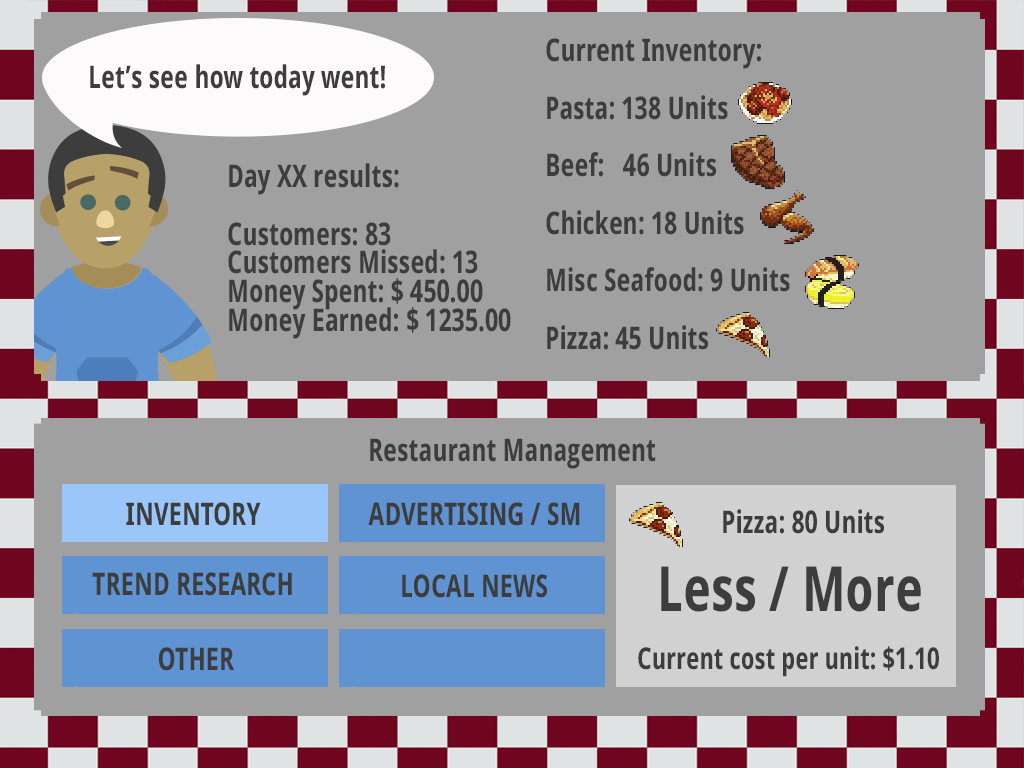
\includegraphics[scale=0.3]{scene2.png}
\caption{Prototype for phase 2 of game where summary of the day is displayed.}
\vspace{5mm}
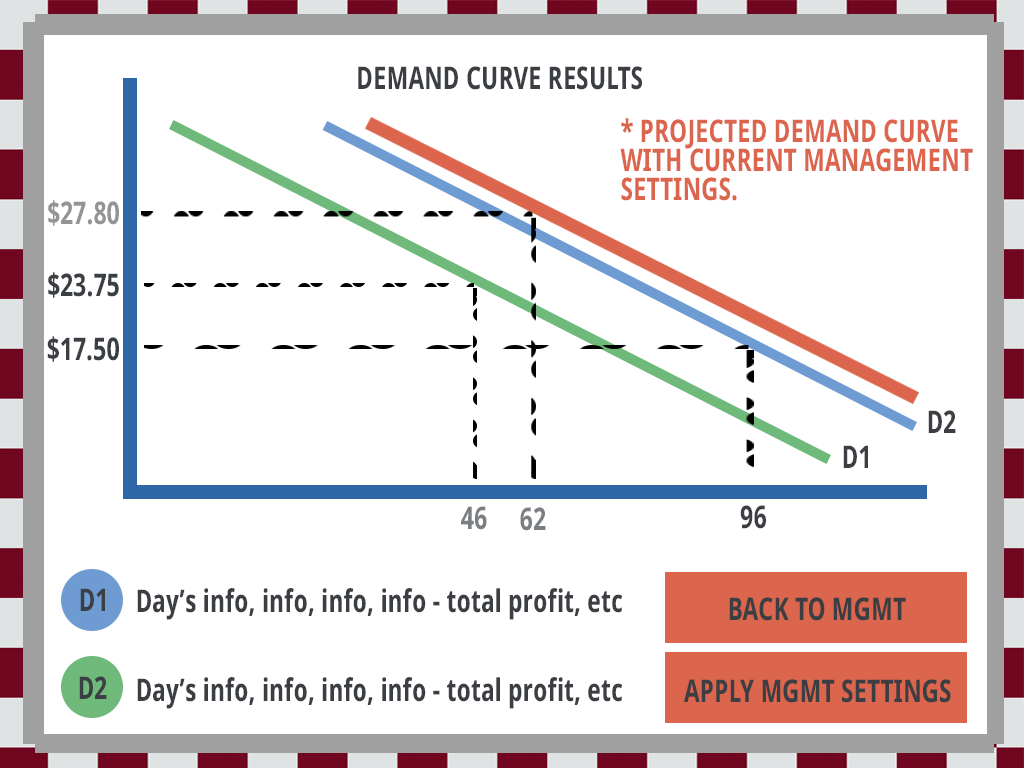
\includegraphics[scale=0.3]{scene2_report.png}
\caption{Prototype for phase 2 of game where demand curve is displayed.}

\end{figure}




\end{document}